\documentclass[12pt]{article}

\usepackage{amsmath, mathtools}
\usepackage{amsfonts}
\usepackage{amssymb}
\usepackage{graphicx}
\usepackage{colortbl}
\usepackage{xr}
\usepackage{hyperref}
\usepackage{longtable}
\usepackage{xfrac}
\usepackage{tabularx}
\usepackage{float}
\usepackage{siunitx}
\usepackage{booktabs}
\usepackage{caption}
\usepackage{pdflscape}
\usepackage{afterpage}
\usepackage{color, colortbl}
\usepackage{float}
\usepackage[round]{natbib}
%\usepackage{helvet}
%\usepackage[none]{hyphenat}
\usepackage{tabularx}
\renewcommand{\familydefault}{\sfdefault}

%\usepackage{refcheck}
	
\definecolor{LightCyan}{rgb}{0.88,1,1}
\hypersetup{
    bookmarks=true,         % show bookmarks bar?
      colorlinks=true,       % false: boxed links; true: colored links
    linkcolor=red,          % color of internal links (change box color with linkbordercolor)
    citecolor=green,        % color of links to bibliography
    filecolor=magenta,      % color of file links
    urlcolor=cyan           % color of external links
}

%% Comments

\usepackage{color}

\newif\ifcomments\commentstrue %displays comments
%\newif\ifcomments\commentsfalse %so that comments do not display

\ifcomments
\newcommand{\authornote}[3]{\textcolor{#1}{[#3 ---#2]}}
\newcommand{\todo}[1]{\textcolor{red}{[TODO: #1]}}
\else
\newcommand{\authornote}[3]{}
\newcommand{\todo}[1]{}
\fi

\newcommand{\wss}[1]{\authornote{blue}{SS}{#1}} 
\newcommand{\plt}[1]{\authornote{magenta}{TPLT}{#1}} %For explanation of the template
\newcommand{\an}[1]{\authornote{cyan}{Author}{#1}}

%% Common Parts

\newcommand{\progname}{ProgName} % PUT YOUR PROGRAM NAME HERE
\newcommand{\authname}{Team \#, Team Name
\\ Student 1 name and macid
\\ Student 2 name and macid
\\ Student 3 name and macid
\\ Student 4 name and macid} % AUTHOR NAMES                  

\usepackage{hyperref}
    \hypersetup{colorlinks=true, linkcolor=blue, citecolor=blue, filecolor=blue,
                urlcolor=blue, unicode=false}
    \urlstyle{same}
                                


% For easy change of table widths
\newcommand{\colZwidth}{1.0\textwidth}
\newcommand{\colAwidth}{0.13\textwidth}
\newcommand{\colBwidth}{0.82\textwidth}
\newcommand{\colCwidth}{0.1\textwidth}
\newcommand{\colDwidth}{0.05\textwidth}
\newcommand{\colEwidth}{0.8\textwidth}
\newcommand{\colFwidth}{0.17\textwidth}
\newcommand{\colGwidth}{0.5\textwidth}
\newcommand{\colHwidth}{0.28\textwidth}

% Used so that cross-references have a meaningful prefix
\newcounter{defnum} %Definition Number
\newcommand{\dthedefnum}{GD\thedefnum}
\newcommand{\dref}[1]{GD\ref{#1}}
\newcounter{datadefnum} %Datadefinition Number
\newcommand{\ddthedatadefnum}{DD\thedatadefnum}
\newcommand{\ddref}[1]{DD\ref{#1}}
\newcounter{theorynum} %Theory Number
\newcommand{\tthetheorynum}{T\thetheorynum}
\newcommand{\tref}[1]{T\ref{#1}}
\newcounter{tablenum} %Table Number
\newcommand{\tbthetablenum}{T\thetablenum}
\newcommand{\tbref}[1]{TB\ref{#1}}
\newcounter{assumpnum} %Assumption Number
\newcommand{\atheassumpnum}{P\theassumpnum}
\newcommand{\aref}[1]{A\ref{#1}}
\newcounter{goalnum} %Goal Number
\newcommand{\gthegoalnum}{P\thegoalnum}
\newcommand{\gsref}[1]{GS\ref{#1}}
\newcounter{instnum} %Instance Number
\newcommand{\itheinstnum}{IM\theinstnum}
\newcommand{\iref}[1]{IM\ref{#1}}
\newcounter{reqnum} %Functional Requirement Number
\newcommand{\frthereqnum}{P\thereqnum}
\newcommand{\frref}[1]{R\ref{#1}}
\newcounter{nfrnum} %NFR Number
\newcommand{\rthenfrnum}{NFR\thenfrnum}
\newcommand{\nfrref}[1]{NFR\ref{#1}}
\newcounter{lcnum} %Likely change number
\newcommand{\lthelcnum}{LC\thelcnum}
\newcommand{\lcref}[1]{LC\ref{#1}}

\usepackage{fullpage}

\newcommand{\deftheory}[9][Not Applicable]
{
\newpage
\noindent \rule{\textwidth}{0.5mm}

\paragraph{RefName: } \textbf{#2} \phantomsection 
\label{#2}

\paragraph{Label:} #3

\noindent \rule{\textwidth}{0.5mm}

\paragraph{Equation:}

#4

\paragraph{Description:}

#5

\paragraph{Notes:}

#6

\paragraph{Source:}

#7

\paragraph{Ref.\ By:}

#8

\paragraph{Preconditions for \hyperref[#2]{#2}:}
\label{#2_precond}

#9

\paragraph{Derivation for \hyperref[#2]{#2}:}
\label{#2_deriv}

#1

\noindent \rule{\textwidth}{0.5mm}

}

\begin{document}

\title{Software Requirements Specification for \progname: An EMA Enabled Activity Tracker and Prompting System}
\author{\authname}
\date{\today}

\maketitle

~\newpage

\pagenumbering{roman}

\tableofcontents
\listoffigures
\listoftables
~\newpage

\section*{Revision History}

\begin{table}[H]
	\begin{tabularx}{\textwidth}{p{4cm}p{2cm}X}
	  \toprule {\bf Date} 		  & {\bf Version}	 & {\bf Notes} \\
	  \midrule
	  October 5th, 2022              & 1.0           		& Initial Revision       \\
	  November 1st, 2022		  & 1.1           		& Added extra sections,new requriements and hyperlinking\\   
	  November 5th, 2022           & 1.2                       & Additional non-functional requirements added pertaining to hazard analysis\\
	  \bottomrule
	\end{tabularx}
	\caption{\label{revHist}Revision History}
\end{table}
~\newpage
\pagebreak
\section{Reference Material}
\label{Ref_Material}
This section records information for easy reference.

\subsection{Table of Units}

Throughout this document SI (Syst\`{e}me International d'Unit\'{e}s) is employed
as the unit system.  In addition to the basic units, several derived units are
used as described below.  For each unit, the symbol is given followed by a
description of the unit and the SI name.
~\newline

\renewcommand{\arraystretch}{1.2}
%\begin{table}[ht]
	\begin{table}[H]
	  \noindent\begin{tabular}{l l l} 
	    \toprule		
	    \textbf{symbol} & \textbf{unit} & \textbf{SI}\\
	    \midrule 
	    \si{\metre} & length & metre\\
	    \si{\kilogram} & mass	& kilogram\\
	    \si{\second} & time & second\\
	    \si{\degree} & angle & degree\\
	    \si{\radian} & angle & radian\\
	    \si{\V} & potential & volts\\
	    \si{\ampere} & current & ampere\\
	    \si{\ohm} & resistance & ohm (\si\ohm = \si{\V\per\ampere})\\
	    \si{\F} & capacitance & farad\\
	    \si{\H} & inductance & henry\\
	    N & force & newton (N = \si{\kilogram\metre\per\square\second})\\
	    Pa & pressure & pascals (Pa = N\si{\per\square\metre})\\
	    \si{\Hz} & frequency & hertz\\
	    \si{\joule} & energy & joule\\
	    \si{\watt} & power & watt (W = \si{\joule\per\second})\\
	    \bottomrule
	  \end{tabular}
	\caption{\label{tabUnit}Table of Basic Units}
	\end{table}  
  ~\newline
Below are some derived units that do not use a specific SI symbol.
~\newline

  \renewcommand{\arraystretch}{1.2}
\begin{table}[H]
	 \noindent \begin{tabular}{l l} 
	    \toprule		
	    \textbf{Derived unit} & \textbf{SI}\\
	    \midrule 
	    area  & \si{\square\metre}\\
	    volume & \si{\cubic\metre}\\
	    velocity &  \si{\metre\per\second}\\
	    acceleration &  \si{\metre\per\square\second}\\    
	    \bottomrule
	  \end{tabular}
	\caption{\label{devUnit}Table of Derived Units}  
\end{table}

\subsection{Table of Symbols}

The table that follows summarizes the symbols used in this document along with
their units.  The choice of symbols was made to be consistent with kinematics and existing documentation of existing activity trackers. The symbols are listed in alphabetical order.

\renewcommand{\arraystretch}{1.2}

\begin{table}[H]
	\noindent\begin{longtable*}{l l p{12cm}} \toprule
	
	\textbf{symbol} & \textbf{unit} & \textbf{description}\\
	\midrule
	$f_c$ & \si{\Hz} & clock frequency of microcontroller\\
	$m_{tracker}$ & \si\g & mass of activity tracker (device)\\
	$a_r$ & \si{\metre\per\square\second} & accelerometer resolution\\
	$A_{tracker}$ & \si[per-mode=symbol] {\square\metre} & estimated area of activity tracker\\
	$V_{battery}$ & \si\V & supplied voltage of battery\\
	
	\bottomrule
	\end{longtable*}
	\caption{\label{symb}Table of Symbols}  
\end{table}

\subsection{Abbreviations and Acronyms}

\renewcommand{\arraystretch}{1.2}
\begin{table}[H]
	\noindent\begin{tabular}{l l} 
	  \toprule		
	  \textbf{symbol} & \textbf{description}\\
	  \midrule 
	  A & Assumption\\
	  ACC & Acceleration\\
	  BAR & Barometer\\
	  CSV & Comma-Separated Values\\
	  CV & Controlled Variables\\
	  DD & Data Definition\\
	  EMA & Ecological Momentary Assessment\\
	  FSM & Finite State Machine\\
	  GD & General Definition\\
	  GS & Goal Statement\\
	  GYR & Gyrometer\\
	  IM & Instance Model\\
	  LC & Likely Change\\
	  LSS & Lumbar Spinal Stenosis\\
	  MV & Monitored Variables\\
	  NFR & Non-Functional Requirements\\
	  OOP & Object Oriented Programming\\
	  PID & Proportional-integral-derivative\\
	  PS & Physical System Description\\
	  R & Requirement\\
	  SI & Syst\`{e}me International d'Unit\'{e}s\\
	  SReS & School of Rehabilitation Sciences\\
	  SRS & Software Requirements Specification\\
	
	  \bottomrule
	\end{tabular}\\
	\caption{\label{abbacr}Table of Abbreviations and Acronyms}  
\end{table}

\subsection{Constants}
Below are the constant that will be used in the device.
\renewcommand{\arraystretch}{1.2}
\begin{table}[H]
	\noindent \begin{longtable*}{l l p{12cm}} \toprule
	
	\textbf{symbol} & \textbf{value and unit} & \textbf{description}\\
	\midrule
	$g$ & 9.81 \si{\metre\per\square\second} & acceleration due to gravity\\
	$f_{ESP32}$ & Adjustable from 80 \si{MHz} to 240 \si{MHz} & clock frequency of ESP32-D0WD chip.\\
	\bottomrule
	\end{longtable*}
	\caption{\label{const}Table of Constants} 
\end{table}


\subsection{Mathematical Notation}
N/A
\pagenumbering{arabic}


\section{Introduction}
\label{Intro}

Researchers at the School of Rehabilitation Sciences (SReS) at McMaster University are investigating treatment strategies for victims of spinal disorders and back pain. Currently, there is great interest in performing Ecological Momentary Assessment (EMA) on those who suffer from back pain and disorders to make treatment options more effective. EMA aims to study the thoughts, experiences, and behaviours of a patient's daily life by repeatedly collecting data in an individual's normal environment, at or close to the time they carry out that behaviour.\\

Specifically, the type of EMA that the SReS is interested in is focused on analyzing the daily activities and symptoms of mostly-older adults with mobility and spinal issues. For example, they may be interested in performing EMA on a patient with spinal compression issues which prevent them from being able to walk long distances without experiencing pain or distress. They wish to track that patient's walking activity as they go about their daily life. If this patient stops walking or moving, they wish to prompt them with questions such as, "Did you stop moving? If so, was it due to pain? Describe your pain, describe which portion of the body it is in." The answers to these questions will be combined with activity monitoring data to form a better picture about the experience this patient has with their spinal and mobility issues.\\

EMA has become an increasingly popular research methodology in the realm of pain related studies. In 2022, the SReS wished to evaluate the feasability of an eHealth-based prehabilitation program for participants undergoing surgery for lumbar spinal stenosis (LSS). ~\cite{MacedoPilotTrial} This study incorporated EMA into the study; With a wearable triaxial accelerometer (Actiwatch Spectrum Pro Startup, Philips, USA) worn for seven days in a row, total weekly minutes of physical activity were recorded. This battery-operated accelerometer captured time-varying accelerations. Data was gathered on maximum duration of continuous exercise, volume of activity (total counts of activities per week), energy expenditure intensities, and maximal intensity (maximum counts of activities per minute). Then for three times a day for seven days, participants were asked to assess how severe their pain and exhaustion were. This data was collated together and used to evaluate the evaluate the effect LSS had on walking ability and daily pain. \\

In order to accomplish this, the researchers have attempted to use various smart-watch-esque activity tracking devices to track the activity of their patients, and have attempted to use apps and different pieces of software for them to prompt their patients with questions. However, they have been frustrated with very limited success, and are looking for a system which integrated precise and relevant activity tracking with user-friendly self-reporting symptom functionality.\\

The researchers require a method to perform EMA analysis in a manner which even older patients can use, integrated into one package which gathers relevant data about a patient's activities and allows them to easily report what is currently going on and how they feel. They also are looking for a way to access EMA data in various ways. This includes graphical representations of the data which are meaningful to researchers, along with the raw data itself. This data could be activity data, symptoms reporting data, both types of data collated together, and so on. \\


This introductory section of the document is intended to provide a reader with an overview of the purpose, overall scope, and organization of the document. As well as a description of the characteristics of the intended reader of this document.\\

\subsection{Purpose of Document}

This document is intended to describe the requirements of Team \#1's system in a structured and collected manner. In other words, this is a document focused on what the system needs to do and the metrics and methods used to measure its performance. This groundwork is laid in a way to allow every individual who reads this document to understand the details essential to the requirements of this system.\\

Additional purposes of this document are to plan for the design stage of the project, foster effective communication between members of the team, and to establish reference material to which team members will be able to refer back to at later stages in the project should they need to acquire a higher-level view of the system.

\subsection{Changes from template}
This document was written based off of the sample work provided in the 4T06 course gitlab page, and changes have been made from the template accordingly. They are included here:\\

\begin{itemize}
	\item Added a constants subheading to section 1. This project does not use the mathematical notation included in the template.
	\item Added a section for users and stakeholders.
	\item Added subsections for monitored and controlled variables.
	\item Renamed Solution Characteristics Specifications to Assumptions, as most of the original Solution Characteristics Specifications is not relevant to this project, other than the 					assumptions section.
	\item Sections 5.2.1 through 5.2.7 are not applicable to this project and have been labelled N/A.
	\item The Development Plan and Value of Auxiliary Constants sections are not applicable to this project and have been labelled N/A.
	\item Added a section for Project Attributes, Normal Operation Overview, Undesirabled Event Handling, and FSM and Dataflow Diagram, and Legal and Regulatory Factors.
\end{itemize}

\subsection{Scope of Requirements}

The scope requirements for a system which satisfies the goals of EMA must be defined properly. In the case of this project, the requirements must include a method of activity monitoring and a way to prompt users with questions relevant to EMA. In addition, this system will be used by older adults in Canada, specifically in a typical Canadian household environment, likely with a fixed daily routine. This system is not intended to be used by bedridden or sedentary users. If a user is unable to maintain a certain level of movement on a regular basis, the entire point of EMA is rendered moot. It is also necessary to exclude children from the sphere of users. This system must be designed for adults, aimed specifically towards older adults.\\

\subsection{Characteristics of Intended Reader} \label{sec_IntendedReader}

While this document is intended to describe the requirements of the system in as abstract of a method as possible, it is unreasonable to expect a layman without any knowledge within the field of mechatronics to understand the contents of this document. Therefore, there are certain characteristics that a reader must have in order to fully grasp the scope of this SRS. \\

A reader should have a grasp of software development, electronics, mechanics and dynamics at a level equivalent to a 3rd-Year Mechatronics Undergraduate University student, as well as a basic understanding of human anatomy of which a high school level is adequate. \\

In addition, a reader should have a high-level understanding of Ecological Momentary Assessment. This does not have to be particularly in depth, but a reader should be able to identify the main objectives, practices, and difficulties of performing EMA. \\

\subsection{Organization of Document}
This document is organized in a way to make it simple for a reader to understand the essentials regarding the requirements of the system. Should one be interested in gaining a general understanding, it is highly recommended to read this document in its entirety. However, should one wish to learn about specific aspects of this project, please feel free to navigate to any individual section as they are each individually comprehensible. If the reader of this document is a participant in the SReS EMA program, the information relevant is located in sections \ref{Intro}, \ref{Users_Stakeholders}, and \ref{GSD}. If the reader of this document is a researcher performing EMA, the information relevant is located in sections \ref{Users_Stakeholders}, \ref{GSD}, \ref{SSD}, \ref{Project_Attr}, \ref{NOO}, and \ref{UEH}.\\ 



%%%%%%%%%%%%%%%%%%%%%%%%%%%%%%%%%%%%%%%%%%%%%%%%%%%%%%%%%%%%%%%%%%%%%%%%%%%%%%%%%%%%
\section{Users and Stakeholders}
\label{Users_Stakeholders}
\begin{itemize}
\item Stakeholders

	\begin{itemize}
		\item  Dr. Luciana Macedo of School of Rehabilitation Science at McMaster University (Primary Project Supervisor).
		\item  Dr. Spencer Smith (Project Supervisor).
	\end{itemize}

\item Stakeholders that are Users: The design has 2 different stakeholders which will be users of the system:
	\begin{itemize}
		\item \textbf{Researchers}: Primary end user who will use the data collected by the device for analysis and research.
		\item \textbf{Patients/Participants} : Users part of the monitoring study who will be wearing the device, and whose activities will be collected for research and analysis.
	\end{itemize}
\end{itemize}
%%%%%%%%%%%%%%%%%%%%%%%%%%%%%%%%%%%%%%%%%%%%%%%%%%%%%%%%%%%%%%%%%%%%%%%%%%%%%%%%%%%%

\section{General System Description}
\label{GSD}
This section provides general information about the system.  It identifies the
interfaces between the system and its environment, describes the user
characteristi	cs and lists the system constraints.  \\\\
\subsection{System Context}

This system in theory is very simple. An array of sensors grabs info regarding the position, speed, orientation, etc. and uses that information to understand the current state of the user. This data is then used to generate prompts that the user will answer and all the collected data is compiled, processed and stored within the system. Finally, researchers will analyze the collected data and generate observations. 
\begin{figure}[h!]

\begin{center}
 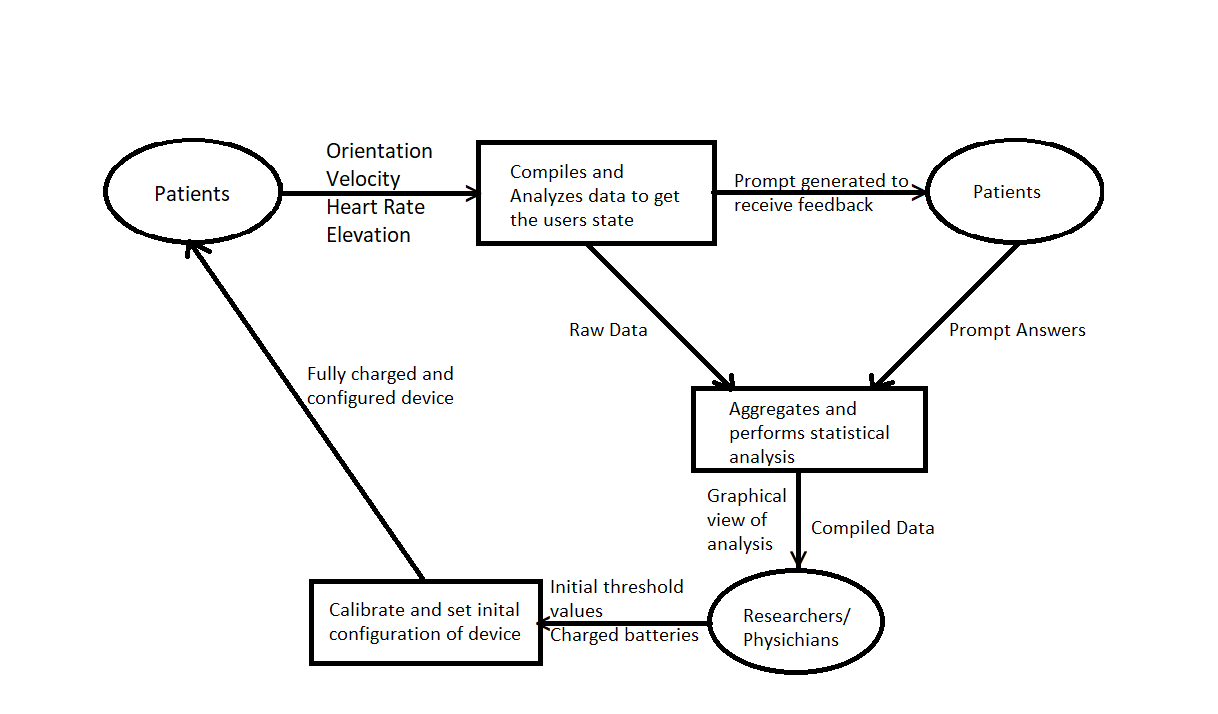
\includegraphics[width=.95\textwidth]{System Context Diagram}
\caption{System Context}
\label{Fig_SystemContext} 
\end{center}
\end{figure}


\begin{itemize}

\item Patient Responsibilities:
\begin{itemize}
\item Patients are required to set up the device correctly so that their various attributes (Orientation, velocity, etc.) can be collected.
\item Patients are also required to answer the prompts given to them so that adequate data can be collected.
\end{itemize}
\item Researcher Responsibilities:
\begin{itemize}
\item Required to confirm that data is being collected.
\item Required to set up the intial thresholds and activities for tracking.
\item Analyze the data.
\item Charge and calibrate the system.
\end{itemize}
\end{itemize}

\subsection{User Characteristics} \label{SecUserCharacteristics}

Patients should have a general understanding of using smart devices with touch-bezel interfaces. Patients will also be required to wear the device on their body so a good understanding of how to setup the device and secure it will be required. Finally the device will prompt users to answer certain prompts, thus knowledge of what to expect and how to respond is required.\\

Researchers will have the option of tweaking the configuration of the device, allowing them to manipulate certain activity thresholds. Thus a working knowledge of the system is required. Moreover, a basic understanding of graphs and statistical analysis will be required to understand the research data collected by the device.\\\\


\subsection{System Constraints}

The design will consist of both a hardware and a software system. The constraints for both systems are as follows:
\begin{itemize}
\item \textbf{Hardware}: 
	\begin{itemize}
		\label{HC1}\item[HC1:] The system must weigh less than 100g to facilitate being lightweight and comfortable.
		\label{HC2}\item[HC2:] The system must have an average battery life of at least 24 hours to facilitate monitoring of the users.
		\label{HC3}\item[HC3:] The dimensions of the system must be quite small with an area lower than 2500mm\textsuperscript{2}.\\
	\end{itemize}

\item \textbf{Software} :
	\begin{itemize}
		\label{SC1}\item[SC1:] The system will have hard time constrainsts so as to store data and prompt users with low latency .
		\label{SC2}\item[SC2:] To maintain privacy, the system will only store data for as long as the EMA study period lasts.
		\label{SC3}\item[SC3:] The system must prompt users based on activities and not based on time of day. 
	\end{itemize}
\end{itemize}


\section{Specific System Description}
\label{SSD}
\subsection{Problem Description} \label{Sec_pd}

Dr. Luciana Macedo investigates treatment strategies for older adults with musculo-skeletal disorders, based on the results reported through Ecological Momentary Assessment (EMA).
The current solution is not very sensitive to slow and subtle movements. It also works on a time-based approach, reporting data after specified intervals. Moreover, the Human Computer Interface is not user-friendly for the targeted audience and the data gathered is difficult to analyze.
The motive is to design a device that is able to capture very minor movements, that could produce data of interest based on the survey results along with a well-designed interface following HCI conventions allowing users to navigate with ease.

\subsubsection{Terminology and  Definitions}

This subsection provides a list of terms that are used in the subsequent
sections and their meaning, with the purpose of reducing ambiguity and making it
easier to correctly understand the requirements:

\begin{itemize}

  \item PID controller: This stands for proportional–integral–derivative controller. It is an instrument used in industrial control applications to regulate temperature, flow, pressure, speed and other process variables.
  \item FSM: This stands for Finite State Machine. An FSM is a machine that can be in a specific state from finite set of states based on previous conditions and inputs.
  \item TFT LCD: It stands for Thin-Film-Transistor Liquid Crystal Display. This is the display screen where data is shown.
  \item MVC: Model-View-Controller. It is a software architectural pattern used to implement user interfaces, data and controlling logic. It separates display from program logic.
  \item Control variables: These are the variables that will be controlled in our implementation and research to avoid their impact.
  \item Monitored variables: These are the variables that will be calculated based on program logic and output as a result.

\end{itemize}
\subsubsection{Monitored variables}
\begin{table}[H]
\begin{tabular}{ |p{9em}|p{25em}|p{6em}| }
  \hline
  \rowcolor{LightCyan}
  \textbf{Monitored Variable}       	& \textbf{Description}                                                                                                                                                                         			 	& \textbf{Units}\\
  \hline
  \label{mBat}m\_ batteryLife      	& This signal is used to monitor the battery life.                                                                                                                                    				& Integer(\%)\\
  \hline

   \label{mMod}m\_ modeUser        	& This signal is used to indicate who is the user. There are only two types of users: participant and researcher. Mode for participant is 0 and 1 for researcher.   	& Boolean \\
  \hline
  \label{mAct}m\_ ActivityDetected  	& This signal is used to monitor the current state of the participant.                                                                                            						& struct(Boolean, Integer)\\
  \hline
  \label{mPro}m\_ promptAnswered   	& This signal is used to monitor the state of the participant response to the activity prompt.                                                                                  			& Boolean\\
  \hline
 \label{mMon} m\_ monitorPer       	& This signal is used to monitor the duration, the participant has been monitored since the device has been turned on.                                        			&Integer (number of days)\\
  \hline
 \label{mVal}m\_ valConnect       	& This signal is used to indicate whether the researcher's system can be validated as a host.                 											& Boolean\\
  \hline

 \label{mSen} m\_ senCalVal        	& This signal is used to indicate whether the sensors have been calibrated successfully according to the researcher's constraints.                                                & Boolean\\
  \hline
\end{tabular}
\\
\linebreak
\linebreak
\caption{\label{monVar}Table of Monitored Variables}  
\end{table}

\subsubsection{Controlled variables}
\begin{table}[H]
\begin{tabular}{ |m{10em}|m{25em}|m{5em}| }
  \hline
  \rowcolor{LightCyan}
  \textbf{Controlled Variable} & \textbf{Description}                                                                                                          & \textbf{Units}           \\
  \hline
  \label{cBat}c\_batteryLife & This is the battery threshold that the battery life should be above to indicate that the device is good for usage             & Integer(\%)              \\
  \hline
  \label{cMon}c\_monitorPer  & This is the monitoring period set for participants by the researcher. The device shall be collecting data within this period. & Integer (number of days) \\
  \hline
  \label{cMod}c\_modeResearcher   & This flag is used to control what the software does. There are 3 different actions: for Calibration, Accessing patient records, and Accessing data collected. & Integer                  \\
  \hline
\end{tabular}
\caption{\label{conVar}Table of Controlled Variables}  
\end{table}
\subsubsection{Comparison to existing solutions}
Most of the solutions are just softwares when installed, uses phone sensor data to cause an intervention. They are very dependent on mobile phone sensors, meaning if there are no sensors on the phone, the software application becomes obsolete.
The app might also have to be open 24/7 or running in background to be able to read live sensor data.  Some of the current solutions involved a time-based EMA trigger
which may cause the data collected to be segregated as the trigger time intervals could be well beyond when the user expressed a desired behaviour.
\\\\
Most of the solutions could include smartwatches such as Fitbit, Samsung Galaxy Watch. These products are not very accurate as they could track movement wrongly, leading to wrong results.
These devices can also be easily tampered by participants, which could affect the results produced in favour of participants.
They also tend to be very expensive due to some features offered, which may not be useful to the situation.
\\\\
The device that we will be designing will be independent of the cellphone devices. This removes the ambiguity in the linking of phone sensors to software application for tracking. It will be collecting data live and triggering EMA based on sensor data, thus being momentary and
more accurate responses are expected to be responded at the time of happening. It will also thrive to use very sensitive sensors, so that every minor movement can be captured, which is limited to the existing solutions due to their dependency on phone sensors.
Some of the softwares could be very expensive despite the limitations they have, such as being dependent entirely on phone. This makes the overall system expensive as the user will need
to be owning a phone which could add to the total expenses. The device that we will be designing is also expected to have longer battery life and ease-of-comfort while wearing. They will have an added layer of security, where the participants cannot recalibrate the devices, hence enhancing accuracy of the results.
It will be very cheap and specific to the purpose, thus ensuring better performance, and higher reliability.
\subsubsection{Physical System Description} \label{sec_phySystDescrip}



\begin{itemize}

  \label{PS1}\item[PS1:] The display screen will be around 2500 mm$^2$. This will be the interface between the user and the system.
  \label{PS2}\item[PS2:] The bracket around the screen will be approximately 2700 mm$^2$. This will be an added layer of protection against the screen to avoid damages to the screen itself.
  \label{PS3}\item[PS3:] The weight of the device will be less than or equal to 100 grams. This is because of the additional weight coming from the straps and embedded sensors. The resultant force will be in the direction of arm, since arm weighs approximately 3.5 kg, making the device lightweight.
  \label{PS4}\item[PS4:] The strap will be approximately 75mm long on the short side and 140 mm long on the long side, so that it sits perfectly and comfortably on the user's wrist.

\end{itemize}


\subsubsection{Goal Statements}
\begin{itemize}

  \label{GS1} \item[GS1:] \textbf{Minor movement tracking}: The idea is to be able to capture very subtle, minor movements, as most activity trackers are incapable of doing it. Since our target audience have limited movements, the device needs to be sensitive to capturing minor motion since that would produce the desired data.
   \label{GS2}\item[GS2:] \textbf{Event-based prompting}: Based on desired trigger events, the user would be prompted to complete the EMA.
   \label{GS3}\item[GS3:] \textbf{Simple User Interface}: We want to be able to design a very intuitive User interface, one that would be very interactive and easy to navigate around. This would result in quicker and more accurate survey submissions as they are prompted.
   \label{GS4}\item[GS4:] \textbf{Graph Representation}: Researchers desire to be able to capture the trends in the behaviours over a set time. Graphical outputs are the best method to capture and understand the behaviour of certain dependent variables.

\end{itemize}

\subsection{Assumptions}%Solution Characteristic specification

\begin{itemize}

\item[A\refstepcounter{assumpnum}\theassumpnum
\label{A1}:]
{All users are fluent English speakers.}

\item[A\refstepcounter{assumpnum}\theassumpnum
\label{A2}:]
{The device is to be used under normal daily activities.}

\item[A\refstepcounter{assumpnum}\theassumpnum
\label{A3}:]

{All patients are to receive verbal instructions from their researcher on how to use their devices.}

\end{itemize}


\subsubsection{Theoretical Models}\label{sec_theoretical}
N/A

\subsubsection{General Definitions}\label{sec_gendef}
N/A
\subsubsection*{Detailed derivation of simplified rate of change of temperature}
N/A

\subsubsection{Data Definitions}\label{sec_datadef}
N/A

\subsubsection{Data Types}\label{sec_datatypes}


N/A



\subsubsection{Instance Models} \label{sec_instance}
N/A

\subsubsection*{Derivation of ...}
N/A

\subsubsection{Input Data Constraints} \label{sec_DataConstraints}
N/A


\subsubsection{Properties of a Correct Solution} \label{sec_CorrectSolution}
N/A


%%%%%%%%%%%%%%%%%%%%%%%%%%%%%%%%%%%%%%%%%%%%%%%%%%%%%%%%%%%%%%%%%%%%%%%%%%%%%%%%%%%%
\section{Required Behavior}
\label{Req_Behavior}
The activity tracking system should have the following required behavior: \\

\begin{itemize}
\item Motion tracking should be accurate and in line with industry standards in activity tracking\\
\item The activity tracker must be able to turn on, or reboot itself without user intervention if an issue is detected\\
\item The battery must last a minimum of 24 hours\\
\item The system must be able to store at least one EMA period's worth of activity tracking data locally\\
\item The system should be intuitive and seamless for the user\\
\end{itemize} 
%%%%%%%%%%%%%%%%%%%%%%%%%%%%%%%%%%%%%%%%%%%%%%%%%%%%%%%%%%%%%%%%%%%%%%%%%%%%%%%%%%%%

\section{Requirements}
\label{Requirements}
This section provides the functional requirements, the business tasks that the
software is expected to complete, and the nonfunctional requirements, the
qualities that the software is expected to exhibit.

\subsection{Functional Requirements}
Below are the functional requirements of the device as well as the rationale.


\begin{center}
\begin{tabular}{|l|p{14cm}|}
 \hline
 R1 \label{R1} & Device stays on during the monitoring period. \\ [0.5ex]
 \hline
 Rationale &  The User/Researcher would want to turn on/off the device when not in use.\\ 
 \hline
\end{tabular}
\end{center}
\hspace{0.5cm}
%%%%%%%%%%%%
% Requirement 2
\begin{center}
\begin{tabular}{|l|p{14cm}|}
 \hline
 R2 \label{R2} (Prority) & Device has to track minor movements of user such that activity is recorded appropriately.\\ [0.5ex]
 \hline
 Rationale &  The device will have to track minor movements as a lot of the participants have limited mobility.\\ 
 \hline
\end{tabular}
\end{center}
\hspace{0.5em}
%%%%%%%%%%%
% Requirement 3
\begin{center}
\begin{tabular}{|l|p{14cm}|}
 \hline
 R3 \label{R3}(Prority) &Device has to notify the user when the software detects a registered activity relavent to EMA standards and that is signficant or promptable.\\ [0.5ex]
 \hline
 Rationale &  The device will have to prompt the user if activity stops to check if they are in pain.\\ 
 \hline
\end{tabular}
\end{center}
\hspace{0.5em}
%%%%%%%%%%%
% Requirement 4
\begin{center}
\begin{tabular}{|l|p{14cm}|}
 \hline
 R4 \label{R4} &The activity tracker/system should be such that the user can attach/wear it on their body.\\ [0.5ex]
 \hline
 Rationale &  The system will be attached to an individual's wrist in order to detect activity.\\ 
 \hline
\end{tabular}
\end{center}
\hspace{0.5em}
%%%%%%%%%%%
% Requirement 5
\begin{center}
\begin{tabular}{|l|p{14cm}|}
 \hline
 R5 \label{R5} &Input thresholds should be customizable in the software of the device in a simplistic manner.\\ [0.5ex]
 \hline
 Rationale & The Researcher should be able to change input thresholds in order to tweak the device's settings.\\ 
 \hline
\end{tabular}
\end{center}
\hspace{0.5em}
%%%%%%%%%%%
% Requirement 6
\begin{center}
\begin{tabular}{|l|p{14cm}|}
 \hline
 R6 \label{R6} (Prority) &The device will store all relavent data every time an activity takes place or a prompt is answered on the device.\\ [0.5ex]
 \hline
 Rationale & The data will have to be stored in the on-board memory of the device so that the researcher can extract it.\\ 
 \hline
\end{tabular}
\end{center}
\hspace{0.5em}
%%%%%%%%%%%
% Requirement 7
\begin{center}
\begin{tabular}{|l|p{14cm}|}
 \hline
 R7 \label{R7} (Prority) &The data stored on the device will be able to be extracted such that the data is interpretable in the form of graphical representation and raw data.\\[0.5ex]
 \hline
 Rationale & The researches require data in formats conducive to conducting clinical EMA studies. These formats are most commonly spreadsheet or graphical forms.\\ 
 \hline
\end{tabular}
\end{center}

\subsection{Likely/Unlikely Changes for Functional Requirements}    
\begin{table}[H]
	\begin{tabularx}{1.05\textwidth} { 
		  | >{\centering\arraybackslash}X 
		  | >{\centering\arraybackslash}X 
		  | >{\centering\arraybackslash}X 
		  | >{\centering\arraybackslash}X | }
		 \hline
		 Requirement & Likelihood of Change& Rationale & Ways to Change \\
		 \hline
		 R1  & Very Unlikely  & Key Implementation & N/A  \\
		 \hline
		 R2  & Likely  &Degree of tracking& Change tracking reesolution.  \\
		 \hline
		 R3  & Very Unlikely  & Key Implementation & N/A  \\
		 \hline
		 R4  & Unlikely  & Key Implementation & N/A  \\
		\hline
		 R5  & Unlikely & Key Implementation &  N/A \\
		 \hline
		 R6  & Very Unlikely  & Key Implementation & N/A  \\
		\hline
		 R7  & Unlikely  & Ensures data reaches Researcher & Method of data storage can be changed.  \\
		\hline
	\end{tabularx}
\caption{\label{likChanges}Table of Likely and Unlikely Changes}  
\end{table}

\subsection{Nonfunctional Requirements}

\noindent \begin{itemize}

\item[NFR1 \label{NFR1}:]
  \textbf{Accuracy:} The accuracy of the data collected during each EMA session by this device must meet the level needed for academic research based on said results. This includes results from sensors capturing participant activity, answers provided by participants from event prompting, timestamps of data inputs, geolocation information, and any other information pertinent to the form of EMA being performed.\\

\underline{Rationale:} Should the EMA data coming from the system be considered inaccurate or incomplete, this system is effectively rendered moot as it is intended to be used in a research setting.\\

\underline{Fit Criterion:} The data recorded, stored, and submitted by the system should be accurate to a level considered satisfactory to standard EMA studies conducted by the SReS.\\


\item[NFR2 \label{NFR2}:] \textbf{Usability:} This system should useable by any individual participant who falls within the categeries defined within the user characteristics section of this document. In addition, this system should be easy to set up, monitor, maintain, and reconfigure by any researcher performing EMA using the device.\\


\underline{Rationale:} As many of the participants may be older adults, they may be unfamiliar with modern activity tracking technology. It is unreasoneable to expect such participants to be able to use the functions of this system unless it is explicitly designed to be useable at any level of experience with technology. Also, we don't wanna waste the time of the researchers or introduce unneccessary complexity into operating this system which may introduce erroneous inputs or data interpretations based on confusing interfaces.\\


\underline{Fit Criterion:} The system's interfaces (both to the researchers and the participants) should fit the guidelines of HCI standards, with an emphasis on making this system more useable for those unfamiliar with modern technology.\\

\item[NFR3 \label{NFR3}:]
  \textbf{Maintainability:} Once completed, the system should be entirely maintenance free for the time period it is used for EMA (7 to 14 days). The participants should not have perform any maintenance actions other than charging the device. during this period, and the researchers at most should have to recharge the batteries of the system again and update the parameters they set for the next set of EMA.\\

\underline{Rationale:} As many of the participants may be older adults, maintenance of this system may be daunting to those unfamilar with modern technology. In addition, any downtime due to maintenance needs during each EMA period will result in a loss of valuable EMA data.\\

\underline{Fit Criterion:} Once activated, the system should perform all of its functions continuously without error for a period of 7 days.\\

\item[NFR4 \label{NFR4}:]
  \textbf{Portability:} The system must be capable of performing its functions of data collection and prompting in any location or situation a participant may find themselves in (within their daily activities). In addition, the system must be constructed in a manner which allows the participant to wear/carry, move, and use the device easily and without hassle.\\

\underline{Rationale:} Ecological Momentary Assessment (EMA) is meant to be performed at almost all points of a participant's daily routine. If the system is bulky, difficult to maneuver around or wear, or heavy, a participant's movement and actions will be hindered and they will be unable to provide EMA data accurately.\\


\underline{Fit Criterion:} Has been tested in each individual environment where EMA will be taking place with satisfactory results regarding its portability.\\


\item[NFR5 \label{NFR5}:]
  \textbf{Cleanability:} Each portion of this device must be capable of being cleaned, sanitized, and made hygenic before and after each period of EMA which it is used for. As each component of the device is constructed and used in a different manner, the different needs each component has in order to render it clean must be considered as well.\\


\underline{Rationale:} In a post-COVID world, maintaining personal hygiene is rightfully considered an important aspect of daily life. It is the responsibility of this devices makers to ensure conditions or practices conducive to maintaining health and preventing disease, especially through cleanliness.\\

\underline{Fit Criterion:} Can be sterilized, cleaned, or treated safely and in a manner satisfactory to the standards of the participants and researchers of the SReS.\\


\item[NFR6 \label{NFR6}:]
  \textbf{Safety:} The system must be designed in a way which prevents any harm or injury (whether it be physical, emotional, or mental) from coming to the participants as a result of the useage of the device and its information collection methods. This includes physical characteristics which prevent immediate injury (removal of sharp objects, useage of soft materials), physical characteristics which prevent long-term adverse health effects (human-safe materials, safe levels of noise production), or any other considerations that need to be taken in order to prevent harm to the participant.\\


\underline{Rationale:} Safety speaks for itself. To put a participant in harms way as a result of the functions of this system would be a gross violation of ethics.\\

\underline{Fit Criterion:} The system conforms to the health and safety standards deemed appropriate by the SReS.\\

\item[NFR7 \label{NFR7}:]
  \textbf{Reusability:} The system must be capable of being reused for an appropriate number of times. This means that the system must be capable of completing its functions without error after each period of EMA without need for significant upkeep other than regular maintenance (cleaning the device, scrubbing data from the system, etc.)\\

\underline{Rationale:} Researchers at the SReS intend to use this system for a vast number of EMA periods, and for multiple different forms of research which EMA may assist with. This system must be designed to be able to sustain its functions for whatever purposes and periods of time which the researchers need.\\

\underline{Fit Criterion:} Can be used for 3 consecutive EMA study periods without need for significant maintenance other than nightly charging.\\

\item[NFR8 \label{NFR8}:]
  \textbf{Privacy:} This system must protect the data collected from the participants from being accessed or distributed to inappropriate entities or people. \\


\underline{Rationale:} Data privacy is a right, and one that must be taken seriously. When revealed to inappropriate people or entities, personal information can be used to negatively affect a participant to a great extent. Preservation of the security of participant's peronal information is therefore essential.\\

\underline{Fit Criterion:} Data is collected, distributed, and then erased from the system according to modern data privacy standards.\\

\item[NFR9 \label{NFR9}:]
  \textbf{Accessibility:} This device must be accessible to any participant who is partaking in EMA. Regardless of disability, mental or physical status, a participant must be capable of utilizing this device for EMA with the full ability to collect and respond to prompts in accordance with EMA principles. This includes designing the system's phyical portion with accessibility needs in mind, along with designing the system's software, user interface, and data collection portions to allow any participant to be able to use it.\\

\underline{Rationale:} If this device is exclusionary to those with special accessibility needs, then it is severly limited in its use for EMA. According to the user characteristics, this device will mostly be used for those suffering from musculo-skeletal disorders, and many of these participants may be suffering from additional disabilities as well.\\

\underline{Fit Criterion:} The system has been verified to perform in accordance to modern accessibility standards, for both the physical component of the system, and the data collection/software component of the system.\\

\item[NFR10 \label{NFR10}:]
  \textbf{Non-Disruptiveness:} The system must be designed in a way which allows participants to provide EMA data without significant impact or change to their activities or daily life. This includes bulky constructions which they must spend effort in considering while moving around, significant visual or auditory disruptions which may startle, distract, or annoy participants, embarassing or aesthetically unpleasant constructs, or any other disturbances that they must make considerations for.\\

\underline{Rationale:} It is of paramount importance that this device does not disrupt the daily activities of participants in order to preserve their dignity, and allow them to perform the necessary tasks of their daily lives. In addition, the less the system disrupts their daily activities, the more accurate the picture will be that the system captures of what those daily acitivities are and their relevance to EMA.\\

\underline{Fit Criterion:} The system must be rated sufficiently non-disruptive to the daily lives of the participants using the system during testing.\\

\item[NFR11 \label{NFR11}:]
  \textbf{Hardware Safety:} The system must be designed with certain saftey criteria in mind. To ensure the hardware is safe is it important that the device have sufficent tollerances for Current, Voltage, and Temperature. Battery protection units will be used in the circuitry in case of high current draw. The battery will have charge protection to prevent overcharging/discharging. Additionally, the intensity of emitted frequencies will be in line with safe levels.\\

\underline{Rationale:} Saftey is a top priority. Causing no harm to society is an important part of an engineers code of ethics. Ensuring that the device can be used safely will inherintly make participants feel safe about the use of the device.\\

\underline{Fit Criterion:} The hardware systems must be designed to ensure that participants are not harmed under normal usage of the device.\\

\item[NFR12 \label{NFR12}:]
  \textbf{Messaging:} The system should be able to deliver messages to the participant on the state of the device. These messages can be in the form of prompts or visual signals using LED indicator lights. They should be intuitive to understand and help particpants solve problems on their own without the assistance of the engineering team or the researchers.\\

\underline{Rationale:} Straightforward messaging can help the partipants better navigate using the device, or may be able to tell them if the device is having an issue.\\

\underline{Fit Criterion:} The goal is under normal operation that messaging will not be necessary. But if the system does malfunction, having associated indications to help diagnose these problems is an important step in making the device user friendly.\\


\item[NFR13 \label{NFR13}:]
  \textbf{Hardware Performance:} Ensuring that the hardware of the device is performing up to expected requirements is important. Some of these performance metrics include the speed of data transfer and the battery life of the device. Specifications have been discussed with researchers by comparing devices like FitBits or Garmin watches with respect to performance and battery life.\\

\underline{Rationale:} Perfomance is not just important as a goal for usability, but it is important to ensure that the data which is being collected can be collected in real-time so that the data is accurate and properly displays to the researchers the information they are trying to gather.\\

\underline{Fit Criterion:} The battery should last beyond the recommended timelines which will be testing during volunteer tests and the data should have a transfer speed that allows for real-time information to be collected and aggregated.\\


\item[NFR14 \label{NFR14}:]
  \textbf{Data Security:} The system must ensure that security of participants data is paramount. Since the device will be handling health records it is important that the device keep the data secured. The data should be well protected so that someone with a high capability in techonlogy would not be able to access the data without a security key.\\

\underline{Rationale:} Health records can be used for malicious reasons, and privacy in general is very important to the particpants.\\

\underline{Fit Criterion:} The data should not be accessible by anyone without a physical security key.\\


\end{itemize}

\section{Traceability Matrices and Graphs}
\label{TMG}

The purpose of the traceability matrices is to provide easy references on what
has to be additionally modified if a certain component is changed. Every time a
component is changed, the items in the column of that component that are marked
with an ``X'' may have to be modified as well. In other words it shows the dependencies 
between different requriements and assumptions in the document. 


\newpage
\noindent
\begin{landscape}
\begin{table}[h!]
	\centering
	\begin{tabular}{|c|c|c|c|c|c}
	\hline
		& \aref{A1}& \aref{A2}& \aref{A3} \\
	\hline          %   1   2    3   4  
	\frref{R1}       &   &   & X  \\ \hline
	\frref{R2}       &   & X&    \\ \hline
	\frref{R3}       & X& X& X  \\ \hline
	\frref{R4}       &   & X& X  \\ \hline
	\frref{R5}       &   &   &    \\ \hline
	\frref{R6}       &   &   &    \\ \hline
	\frref{R7}       & X&   &     \\ \hline
	\nfrref{NFR1} &   & X&    \\ \hline
	\nfrref{NFR2} & X& X& X \\ \hline
	\nfrref{NFR3} &   &   &     \\ \hline
	\nfrref{NFR4} &   & X&     \\ \hline
	\nfrref{NFR5} &   X&   &      \\ \hline
	\nfrref{NFR6} &   &  X &X     \\ \hline
	\nfrref{NFR7} &   &  X &     \\ \hline
	\nfrref{NFR8} &  X &   &X     \\ \hline
	\nfrref{NFR9} & X  &   &X      \\ \hline
	\nfrref{NFR10}&  & X  &      \\
	\hline
	\end{tabular}
	\caption{Traceability Matrix Showing the Connections between Assumptions and Other Items}
	\label{Table:A_trace}
\end{table}
\end{landscape}

\begin{table}[h!]
	\centering
	\begin{tabular}{|c|c|c|c|c|c|c|c|}
	\hline
		& \frref{R1}& \frref{R2}& \frref{R3}& \frref{R4}& \frref{R5}& \frref{R6}& \frref{R7} \\
	\hline                    %1   2   3    4   5   6    7   8    9  10  
	\nfrref{NFR1}         &   & X& X&   &   &   & X\\ \hline
	\nfrref{NFR2}         & X&   & X& X&  X&   & X\\ \hline
	\nfrref{NFR3}         & X&   &   &   &   & X&   \\ \hline
	\nfrref{NFR4}         &   & X&   & X&   &   &   \\ \hline
	\nfrref{NFR5}         &   &   &   &  X &   &   &   \\ \hline
	\nfrref{NFR6}         &  X &  X &   &  X &   &   &   \\ \hline
	\nfrref{NFR7}         &   &   &   & X  &   &   &X   \\ \hline
	\nfrref{NFR8}         &   &   X&   &   &   & X  &X   \\ \hline
	\nfrref{NFR9}         &   X&   &   &   &   &   &   \\ \hline 
	\nfrref{NFR10}       &  X &   & X  & X  & X  &   &   \\ 
	\hline
	\end{tabular}
	\caption{Traceability Matrix Showing the Connections Functional Requirements and Non-Functional Requirements}
	\label{Table:R_trace}

\end{table}

The purpose of the traceability graphs is also to provide easy references on
what has to be additionally modified if a certain component is changed.  The
arrows in the graphs represent dependencies. The component at the tail of an
arrow is depended on by the component at the head of that arrow. Therefore, if a
component is changed, the components that it points to should also be
changed.

\section{Development Plan}
\label{Dev_Plan}

\href{https://github.com/zakerl/Capstone_Project/blob/main/docs/DevelopmentPlan/DevelopmentPlan.pdf}{The development plan is available at this link.}

\section{Values of Auxiliary Constants}
\label{VAC}
N/A


%%%%%%%%%%%%%%%%%%%%%%%%%%%%%%%%%%%%%%%%%%%%%%%%%%%%%%%%%%%%%%%%%%%%%%%%%%%%%%%%%%%%
\section{Project Attributes}
\label{Project_Attr}
This is a comphrehensive list of the various Open Issues, Costs and Risks involved with the project. This will be updated to reflect changes in the Design. Moreover this section also includes some stretch goals that may be accomplised depending on the pace and scale of the project.
\begin{itemize}
\item Open Issues:
	\begin{itemize}
		\item A decision must be made whether the design will be worn on the wrist like a smart watch or on the waist like a belt.
		\item Sensor choices must be decided for optimal state detection of the user.
		\item Data transfer protocol must be decided, (Bluetooth, Ethernet, Wifi etc.)
		\item Cost analysis must be performed to see whether designing a custom PCB would be economical.
	\end{itemize}
	

\item Costs:
		\begin{center}
		\begin{table}[H]
			\begin{tabular}{ |c|c|c| } 
				 \hline
				 	\textbf{SNo.} &  \textbf{Item.} &  \textbf{Cost (\$CAD)} \\ 
				 \hline
				 	1 & Arduino Nano 											& \$10 \\ 
				 \hline		
				 	2 & MPU6050 (Accelerometer/ Gyroscope)						& \$12/unit \\ 
				 \hline
				 	3 & BMP-388 (Barometer) 									& \$2.5/unit \\ 
				 \hline
				 	4 & XD-58C (Heart Rate Sensor)								& \$3\\ 
				 \hline
				 	5 & STM32f405rgt6 (Primary Control Chip) 						& \$8/unit \\ 
				 \hline
				 	6 & Electrical Components (Diodes, Resistors, Capacitors ,etc.) 		& \$20 \\ 
				 \hline
				 	7 & Lipo Battery 											& \$30 \\ 
				 \hline
				 	8 &OLED mini display										& \$15 \\ 
				 \hline
				 	9 & Structural Materials (MDF, PLA plastic, wood, etc.) 			& \$10 \\ 
				 \hline
				 	& \textbf{Average Total Cost}								& \$110.5 \\ 
				 \hline
			\end{tabular}
		\caption{\label{bom}Bill of Materials}  
		\end{table}
		\end{center}

\item Risks:
	\begin{itemize}
		\item Battery life will degrade over time.
		\item Device is not sanitized between different monitoring periods.
		\item Device is improperly calibrated causing improper data collection.
		\item User error when answering prompts.
		\item Internal memory storage may become full if redundant data isnt regularly removed.
	\end{itemize}

\item Stretch goals: Detailed explanations of the following are provided in the Specification/Problem Statement Document.
	\begin{itemize}
		\item Detection of Anomalous behaviour may be added to track irregular movements.
		\item Geotagging location of the activities being tracked to achieve observations about high traffic activity areas.
		\item To optimize charging the device, a movement based charging system may be implemented.
	\end{itemize}
\end{itemize}
%%%%%%%%%%%%%%%%%%%%%%%%%%%%%%%%%%%%%%%%%%%%%%%%%%%%%%%%%%%%%%%%%%%%%%%%%%%%%%%%%%%%

%%%%%%%%%%%%%%%%%%%%%%%%%%%%%%%%%%%%%%%%%%%%%%%%%%%%%%%%%%%%%%%%%%%%%%%%%%%%%%%%%%%%
\section{Normal Operation Overview}
\label{NOO}
\setlength{\parindent}{20pt}
Initially, the researcher will connect to the device using the provided software and either register a new participant or select a pre existing participant profile. Once a participant is selected, the researcher can set the thresholds, activities to be tracked and the monitoring period. \\

Once the device is handed off to the participant, an inital set up process is done, where the device is worn by the user and a test prompt is sent. Once this initial set up process is done, the user will simply carry on with their normal day to day and the device will track all registered activities using the onboard sensors. As the data is collected, it is logged into the internal memory and is stored based on the date and time of entry. The user will then remove the device nightly after their daily routine, and charge it for the next day's use.\\

Finally after the monitoring period is finished, the device will go into an idle state until it is returned to the researcher. The researcher will then log in using their master credentials at which point the device will off load all data into the host software which will compile and present the data in a graphical manner.
%%%%%%%%%%%%%%%%%%%%%%%%%%%%%%%%%%%%%%%%%%%%%%%%%%%%%%%%%%%%%%%%%%%%%%%%%%%%%%%%%%%%

%%%%%%%%%%%%%%%%%%%%%%%%%%%%%%%%%%%%%%%%%%%%%%%%%%%%%%%%%%%%%%%%%%%%%%%%%%%%%%%%%%%%
\section{Undersired Event Handling}
\label{UEH}
\begin{itemize}
	\item \textbf{Incorrect start up prompt response}: When the device is turned on by the user for the first time. A simple start up prompt is given just to check that system booted correctly ("Is this device on?"). If the user incorrectly enters their responsem, the system will simply 				perform a quick restart and ask the same question again.

	\item \textbf{Stagnant sensor data}: Should the device store the same sequence of data for an extended period of time, the system will perform a soft reboot of the sensor array to try to fix the issue. If the problem persists, An alert will be sent out to the researchers informing them 			of a system failure.

	\item \textbf{Improper prompt request}: Should the device generate a prompt whe no activity is being conducted. The user can simply report the prompt and the sytem will record an error, perform a soft reboot and continue normal operation.

	\item \textbf{Early battery failure}: The device's battery should normally last 24 hours. If the charge goes below a predefined threshold before the monitoring period ends, activity tracking will cease and the user will be prompted to charge the device.
\end{itemize}

%%%%%%%%%%%%%%%%%%%%%%%%%%%%%%%%%%%%%%%%%%%%%%%%%%%%%%%%%%%%%%%%%%%%%%%%%%%%%%%%%%%%




%%%%%%%%%%%%%%%%%%%%%%%%%%%%%%%%%%%%%%%%%%%%%%%%%%%%%%%%%%%%%%%%%%%%%%%%%%%%%%%%%%%%
\pagebreak
\section{FSM and Dataflow Diagram}
\label{FSM_Dataflow}
\begin{figure}[h!]
	\begin{center}
		 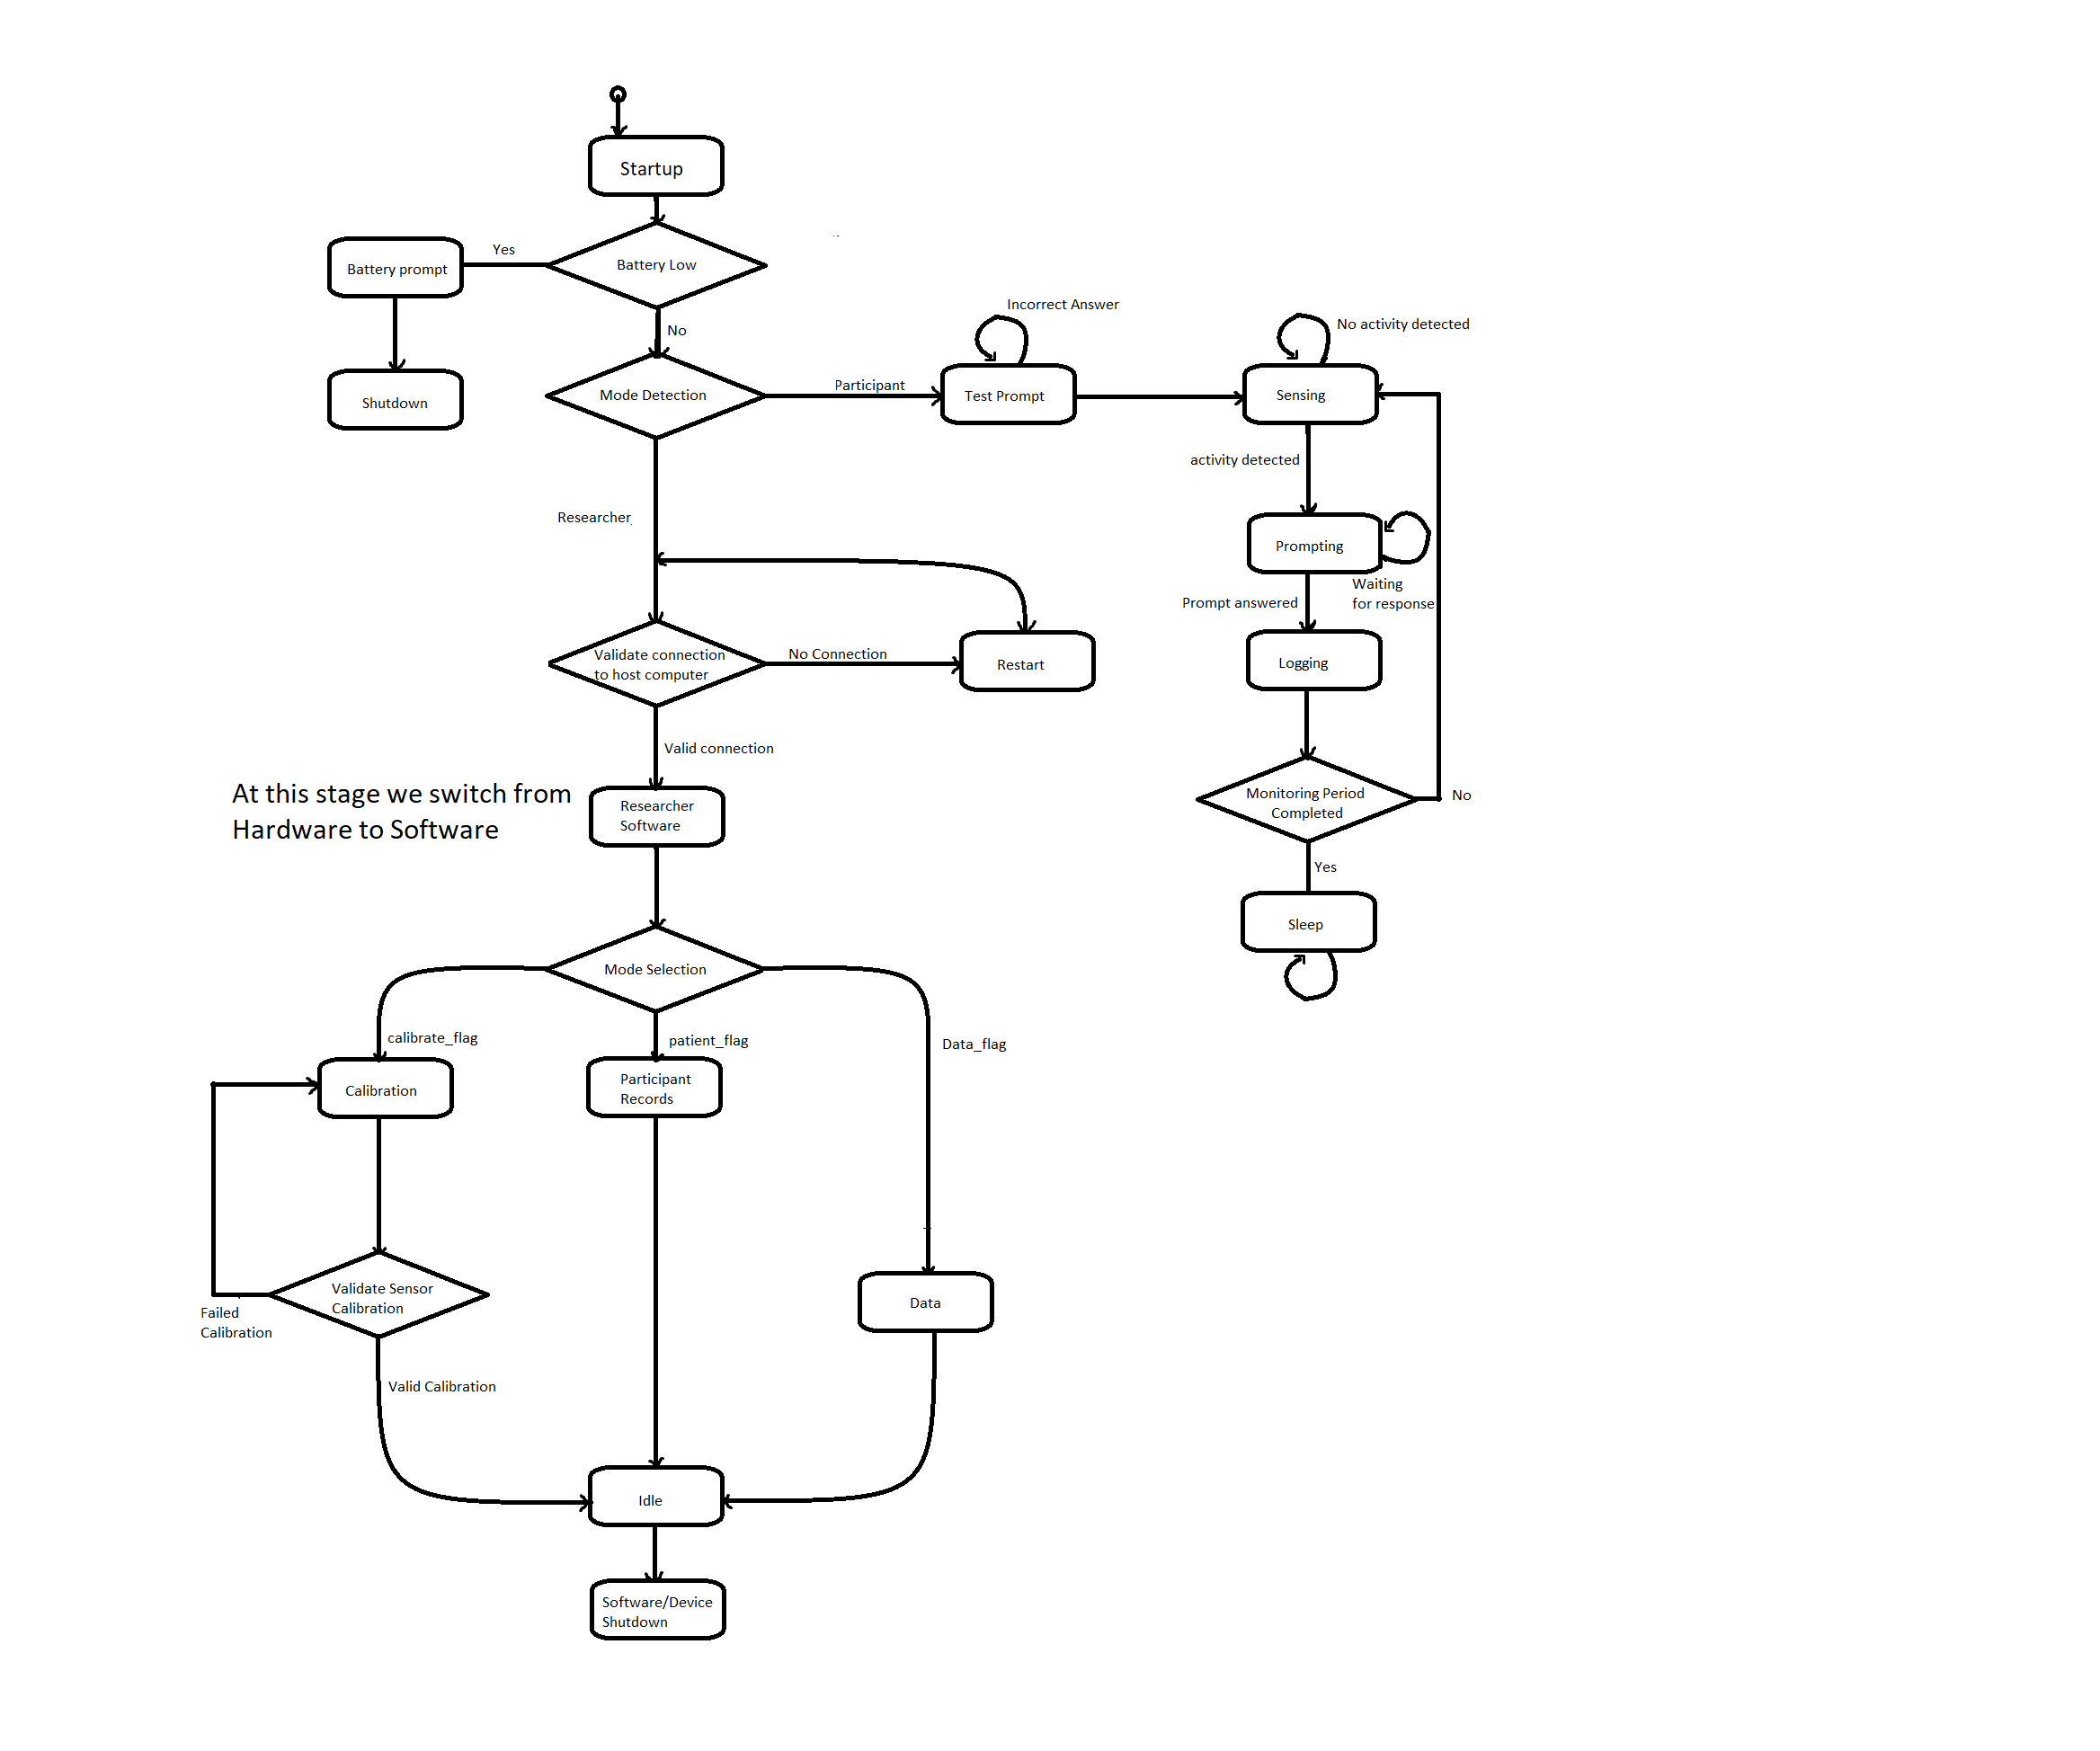
\includegraphics[width=1.3\textwidth]{FSM}
		\caption{FSM}
		\label{Fig_FSM} 
	\end{center}
\end{figure}
The following explains the states presented in the above Finite State Machine:
\begin{itemize}
\item \textbf{States}:
	\begin{enumerate}
		\item \textbf{Startup}: Initial state of the system when it turns on. Simply transitions after checking battery life.           
		\item \textbf{Battery Prompt}: Sends a prompt to the user informing them that the device needs to be charged.
		\item \textbf{Shutdown}: This essentially powers of the device if the battery gets too low. 
		\item \textbf{Test Prompt}: Testing the prompting system by giving a simple question to the user, Is the device on?
		\item \textbf{Sensing}: Reads data from all the sensor and checks whether an activity is detected.
		\item \textbf{Prompting}: Sends a prompt to the user when a registered activity is found. 
		\item \textbf{Logging}: Logs prompt answers and sensor data in the internal memory.
		\item \textbf{Sleep}: Temporarily puts the device to sleep until it is returned to the researchers.
		\item \textbf{Restart}: Restarts the device without going through the startup sequence.
		\item \textbf{Researcher Software}: Initilal state of the software on the host computer. Consists of a simple welcome screen.
		\item \textbf{Calibration}: Calibrates sensors, allows setting new thresholds and choosing what activities to track.
		\item \textbf{Participant Records}: Allows creating and modifying participant information.
		\item \textbf{Data}: Presents all data stored on the device in a graphcial manner.
		\item \textbf{Idle}: Idle state of the software. Awaits any user input.
		\item \textbf{Software/Device shutdown}: When the software shuts down, the device also turns off.
	\end{enumerate}
\end{itemize}
%%%%%%%%%%%%%%%%%%%%%%%%%%%%%%%%%%%%%%%%%%%%%%%%%%%%%%%%%%%%%%%%%%%%%%%%%%%%%%%%%%%%

%%%%%%%%%%%%%%%%%%%%%%%%%%%%%%%%%%%%%%%%%%%%%%%%%%%%%%%%%%%%%%%%%%%%%%%%%%%%%%%%%%%%
\section{Legal and Regulatory Factors}
\label{Legal}

\begin{itemize}
	\item All collected and analyzed non-medical data shall be protected under the Personal Information Protection and Electronic Documents Act (PIPEDA).
	\item All medical records shall be protected under the Personal Health Information Protection Act (PHIPA).
	\item All patients are to sign a waiver form consenting to the use of their personal information and medical records prior to using the device.
	\item Only those with administrative rights will have access to all data files, all data to be secured with passwords.
	\item Documentation to follow IEEE format for references and citations.
	\item Documentation to be completed with 12pt Arial font on US Letter size paper (8.5" x 11") with 1 inch margin on all sides.
	\item The User Interfaces will follow guidelines outlined by the The Accessibility for Ontarians with Disabilities Act (AODA).
\end{itemize}
%%%%%%%%%%%%%%%%%%%%%%%%%%%%%%%%%%%%%%%%%%%%%%%%%%%%%%%%%%%%%%%%%%%%%%%%%%%%%%%%%%%%

\section{Phase in Plan}
\label{Phase_In}

\begin{itemize}
\item October 19: R2: Device has to track minor movements of user such that activity is recorded appropriately.\\
\item October 26: R3: Device has to prompt the user when the software detects no movement has occurred.\\
\item November 02:  R6: The device will have to store data every time an activity takes place or a prompt is answered on the device by the user.\\
\item November 06:  R7: The data stored on the device will have to be extracted such that the data is interpretable in the form of graphs and csv.\\
\end{itemize}
\newpage


\section{References}
\label{References}
N/A
\bibliographystyle {plainnat}
\bibliography {../../refs/References}

\section*{Appendix --- Reflection}

The information in this section will be used to evaluate the team members on the
graduate attribute of Lifelong Learning.  Please answer the following questions:

\begin{enumerate}
  \item \textit{What knowledge and skills will the team collectively need to acquire to
        successfully complete this capstone project?  Examples of possible knowledge
        to acquire include domain specific knowledge from the domain of your
        application, or software engineering knowledge, mechatronics knowledge or
        computer science knowledge.  Skills may be related to technology, or writing,
        or presentation, or team management, etc.  You should look to identify at
        least one item for each team member.}\\

	As the team is still in the burgeoning phases of this project, it is difficult to ascertain the specific "holes" in the team member's specific skillsets that will need to be filled in order to complete this project successfully. However, the time the team has spent working together in the documentation phase has revealed much about what this team requires in order to succeed. \\

As in many multidisciplinary technical projects, diversity of skills translates to strength. In this case, that diversity stretches past knowledge in dispirate technical fields, and extends to areas such as management and business ideation.\\

Obviously, a mechatronics project involving designing wearable technology like this from the ground up requires skills in \textbf{electronics, software engineering, mechanics, and systems design.} Each of which are shared between the team members. While some team members have some experience in these fields (often through internships where team members delved deep into individual skills), there is still catching up to do in order to have the skills necessary to complete the project. After discussion, the team has decided to split these skills among themselves.\\

It is also essential to this project to hone non-technical skills. Without \textbf{effective project management and git management}, this project will fall apart. Project management in this case refers not only to the soft skills (such as effective communication, risk management, time management, etc.), it also refers to the mindset of a project manager working on an extremely time-sensitive and labour intensive project with limited resources. This mindset is often unfortunately learned through failure and hard lessons learned, but the team hopes to pre-emptively practice and hone this. Regarding git management, git is an incredibly powerful tool. However, it is an incredibly powerful tool with a steep learning curve. While this is a skill which is ideally learned by all, the team has identified a specific git leader to learn the specific nuances of git to keep the team out of trouble. \\
	
	These skills-to-be-learned have been split between team members:

	\begin{itemize}
	\item \textbf{Jessica:} Electronics
	\item \textbf{Oliver:} Project Management
	\item \textbf{Jonathan:} Mechanics
	\item \textbf{Anish:} Software Engineering
	\item \textbf{Nish:} Systems Design
	\item \textbf{Labeeb:} Git Nuances
	\end{itemize}
  \item \textit{For each of the knowledge areas and skills identified in the previous
        question, what are at least two approaches to acquiring the knowledge or
        mastering the skill?  Of the identified approaches, which will each team
        member pursue, and why did they make this choice?}
	\begin{itemize}
	\item \textbf{Electronics:}
		\begin{enumerate}
		\item Review the datasheets of microprocessors and circuits previously used in classes.
		\item Attempt to build simplistic projects from online sources using electronics relevant to this project.
		\end{enumerate}
	\item \textbf{Project Management:}
		\begin{enumerate}
		\item Chair all meeting going forward.
		\item Interact with the stakeholders of this project in a leadership role.
		\end{enumerate}
	\item \textbf{Mechanics:}
		\begin{enumerate}
		\item Attempt to try on existing wearable technology and learn the limitations with current technology.
		\item Identify and analyze the material properties of common wearable technology and understand the theory behind their specific applications.
		\end{enumerate}
	\item \textbf{Software Engineering:}
		\begin{enumerate}
		\item Practice with linters, measuring tools for code, and additional software libraries relevant to this project.
		\item Strictly enforce coding requirements to the rest of the team.
		\end{enumerate}
	\item \textbf{Systems Design:}
		\begin{enumerate}
		\item Generate "overviews" of the project, its interactions with the world around it, and the relevancy it has to society.
		\item Simplify all components of the device into a list/diagram which details the interactions each component has with each other and the inputs and outputs of the system.
		\end{enumerate}
	\item \textbf{Git Nuances:}
		\begin{enumerate}
		\item Be "brave" when it comes to using git, github, git issues, and anything relevant to version control. Try weird things!
		\item Begin to implement basic CI/CD with git issues, or with an alternative service if necessary.
		\end{enumerate}
	\end{itemize}
\end{enumerate}

\end{document}